\documentclass[12pt,a4paper]{scrartcl}
\usepackage{scrlayer-scrpage}
\pagestyle{scrheadings}
\ohead{Baumann Martin, 01527563}
\ihead{MLA Homework 4 Report}

\usepackage{lmodern}
\usepackage{float}
\usepackage{listings}

\usepackage{graphicx}
\usepackage{subfig}
\usepackage[T1]{fontenc}
\usepackage{diagbox}
\usepackage{mathtools}

\usepackage{epstopdf}
\usepackage{amsmath}
\usepackage{amssymb}
\usepackage{siunitx}
\sisetup{exponent-product = \cdot, output-product = \cdot}
\usepackage{prettyref}
\newrefformat{fig}{Figure \ref{#1}}
\newrefformat{tab}{Table \ref{#1}}
\newrefformat{eq}{(\ref{#1})}

\usepackage{multirow}
\newcommand{\matr}[1]{\mathbf{#1}}

\usepackage{physics}
\usepackage{tikz}

\begin{document}
	
	\section*{Problem 4.1}
	
	A operation performed by a convolutional layer is technically a cross-correlation and not a convolution, as the name would suggest. For symmetric filters these two operations are equivalent. Nevertheless in machine learning it is often called convolution and therefore I will call it a convolution in the following sections. 
		
	\subsection*{Convolution Input Output Relation}
	
	First, a 1D convolutional layer with nonlinear activation $\sigma(\cdot)$ two filters $\matr{w}^{(0)}$ and $\matr{w}^{(1)}$ with one channel input $\matr{x}$ is considered. 
	The two output channels are given by
	\begin{align}
		z_k^{(0)} &= \sigma\left(\sum_{m=0}^{M-1} w_m^{(0)} x_{k+m} + b^{(0)} \right) \\
		z_k^{(1)} &= \sigma\left(\sum_{m=0}^{M-1} w_m^{(1)} x_{k+m} + b^{(1)} \right).
	\end{align}
	The nonlinear function is applied to the convolution of the input with the corresponding filter and an added bias term. 		
	The input shape in TF is $(b,n,c_\mathrm{i})$ where $n$ is the sequence length, $b$ the batch size and $c_\mathrm{i}$ the number of input channels.
	The weights have the TF shape $(M,c_\mathrm{i},c_\mathrm{o})$ with the filter length $M$ and the number of output channels $c_\mathrm{o}$.
	The convolution can be thought of as sliding the filter along the sequence and summing up all the element wise multiplications. The strides argument controls by how many positions the filter is moved to the right at each step. The output sequence length gets smaller when strides is set to a higher value.
	
	
	Secondly, a 1D convolution layer with nonlinear activation $\sigma(\cdot)$ one filter $\matr{w}$ and two channel input $\matr{x}^{(0)}$, $\matr{x}^{(1)}$ is considered.
	Now only one output channel is produced
	\begin{equation}
		z_k^{(0)}  = \sigma\left( \sum_{j=0}^{c_\mathrm{i}-1} \sum_{m=0}^{M-1}  w_{m}^{(j)} x_{k+m}^{(j)} + b\right).
	\end{equation}
	The shapes mentioned above apply here too, $c_\mathrm{i}=2$ and $c_\mathrm{o}=1$ in this case.
	
	Lastly, a 2D convolution layer with nonlinear activation $\sigma(\cdot)$ one filter $\matr{W}$ and one channel input $\matr{X}$ is considered.
	\begin{equation}
		Z_{k,j} = \sigma\left(\sum_{m_1=0}^{M_\mathrm{h}-1} \sum_{m_2=0}^{M_\mathrm{w}-1} W_{m_1,m_2} X_{k+m_1,j+m_2} + b \right)
	\end{equation}
	The input as well as the filter are now two dimensional. The summation runs over height $M_\mathrm{h}$ and width $M_\mathrm{w}$ of the filter.
	The TF input shape is $(b,h_\mathrm{i},w_\mathrm{i},c_\mathrm{i})$ corresponding to batch size, height, width and number of channels on the input.
	The TF weight shape is $(M_\mathrm{h},M_\mathrm{w},c_\mathrm{i},c_\mathrm{o})$.
	Strides can now be set independently for height and width, the interpretation is again the same but the filter is slid across both dimensions of the input.
	
	\subsection*{Backpropagation}
	
	Considering the MSE loss function 
	\begin{equation}
		J\left(\matr{y}, \matr{w}, \matr{x}\right) = \frac{1}{K} \sum_{k=1}^{K} \left(y_k-z_k \right)^2
	\end{equation}
	and a 1D convolution with linear activation, where the second sum was obtained by a change of summation variable
	\begin{equation}
		z_k = \sum_{m=0}^{M-1} w_m x_{k+m} + b = \sum_{l=k}^{k+M-1} x_l w_{l-k} + b
	\end{equation}
	the partial derivates of the loss and the convolution output are given by
	\begin{align}
		\frac{\partial J}{\partial z_k} &= \frac{2}{K} \left(z_k-y_k\right) \\
		\frac{\partial z_k}{\partial w_m} &= x_{k+m} \\
		\frac{\partial z_k}{\partial x_l} &= w_{l-k}
	\end{align}

	The gradient of the loss is now affected by multiple elements and is therefore given by a summation
	\begin{align}
		\frac{\partial J}{\partial w_m} &= \sum_{k=1}^{K} \frac{\partial J}{\partial z_k} \frac{\partial z_k}{\partial w_m} = \frac{1}{K} \sum_{k=1}^{K} 2\left(z_k-y_k\right) x_{k+m} \label{eq:grad1} \\
		\frac{\partial J}{\partial x_l} &= \sum_{k=1}^{K} \frac{\partial J}{\partial z_k} \frac{\partial z_k}{\partial x_l} = \frac{1}{K} \sum_{k=1}^{K} 2\left(z_k-y_k \right)w_{l-k} \label{eq:grad2}
	\end{align}
	
	Mathematically the gradient in \prettyref{eq:grad1} is a cross-correlation, the gradient in \prettyref{eq:grad2} is now a true convolution.

	\subsection*{Image Filtering}
	
	The two filters 
	
	\begin{equation}
		\matr{W}_{(0)} = \begin{bmatrix*}[r]
			-1 & 0 & 1 \\ -2 & 0 & 2 \\ -1 & 0 & 1
		\end{bmatrix*} \qquad
		\matr{W}_{(1)} = \begin{bmatrix*}[r]
		-1 & -2 & -1 \\ 0 & 0 & 0 \\ 1 & 2 & 1
	\end{bmatrix*} \qquad
	\end{equation}
	
	were applied to the original images in \prettyref{fig:ex4_1_img_orig}.
	
	The outputs are shown in \prettyref{fig:ex4_1_img_filt}.
	The first filter acts like a differentiation in horizontal direction, the second one like a differentation in vertical direction.
	For the edges image the first filter produced an output in response to the left and right edges, the second filter in response to the upper and lower edges and the white bar in the center.
	Looking at the filtered left edge, it can be seen that the output is a white line followed by a black line (going from left to right).  This is due to the white line on the black background in the original image. When differentiated it produces a positive value followed by a negative value.
	
	In the filtered bike images it can be seen that the first filter highlights the vertical edges of the tiles in the background. The second filter highlights the horizontal edges.
	
	\begin{figure}[H]
		\centering	
		\subfloat[Edges]{
\includegraphics[height=0.25\linewidth]{figs/edges.png}}
		\subfloat[Bike]{	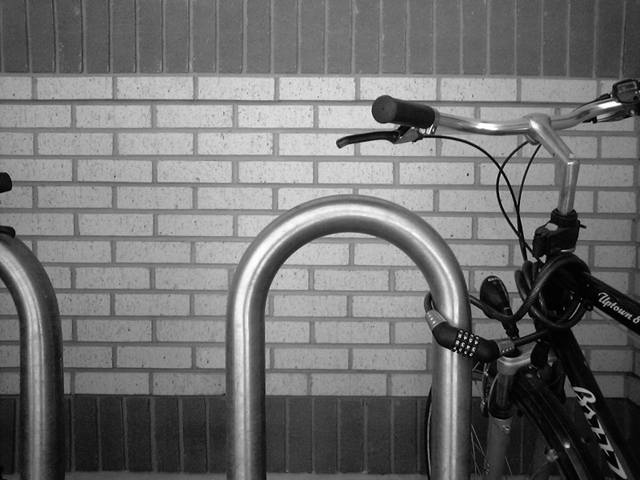
\includegraphics[height=0.25\linewidth]{figs/bike.png}}
		\caption{Original images}
		\label{fig:ex4_1_img_orig}
	\end{figure}

	\begin{figure}[H]
		\centering	
		\subfloat[Edges]{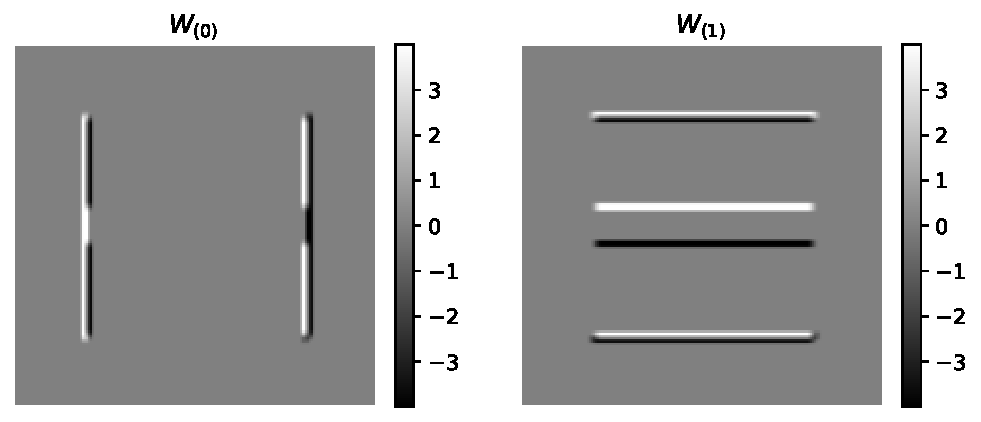
\includegraphics[width=0.7\linewidth]{figs/ex4_1_filt_edges}} \\
		\subfloat[Bike]{	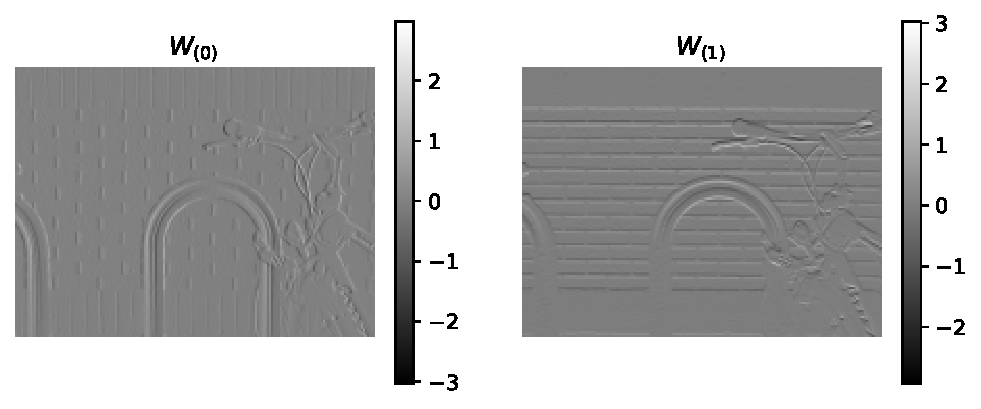
\includegraphics[width=0.8\linewidth]{figs/ex4_1_filt_bike}}
		\caption{Filtered images}
		\label{fig:ex4_1_img_filt}
	\end{figure}

\section*{Problem 4.2}
	
	\subsection*{Dataset}
	
	A random sample of all of the classes are shown in \prettyref{fig:ex4_2_digits} with the class label annotated on the top.
	For training the neural network the class labels where converted to a one hot encoding.
	
	\begin{figure}[H]
		\centering
		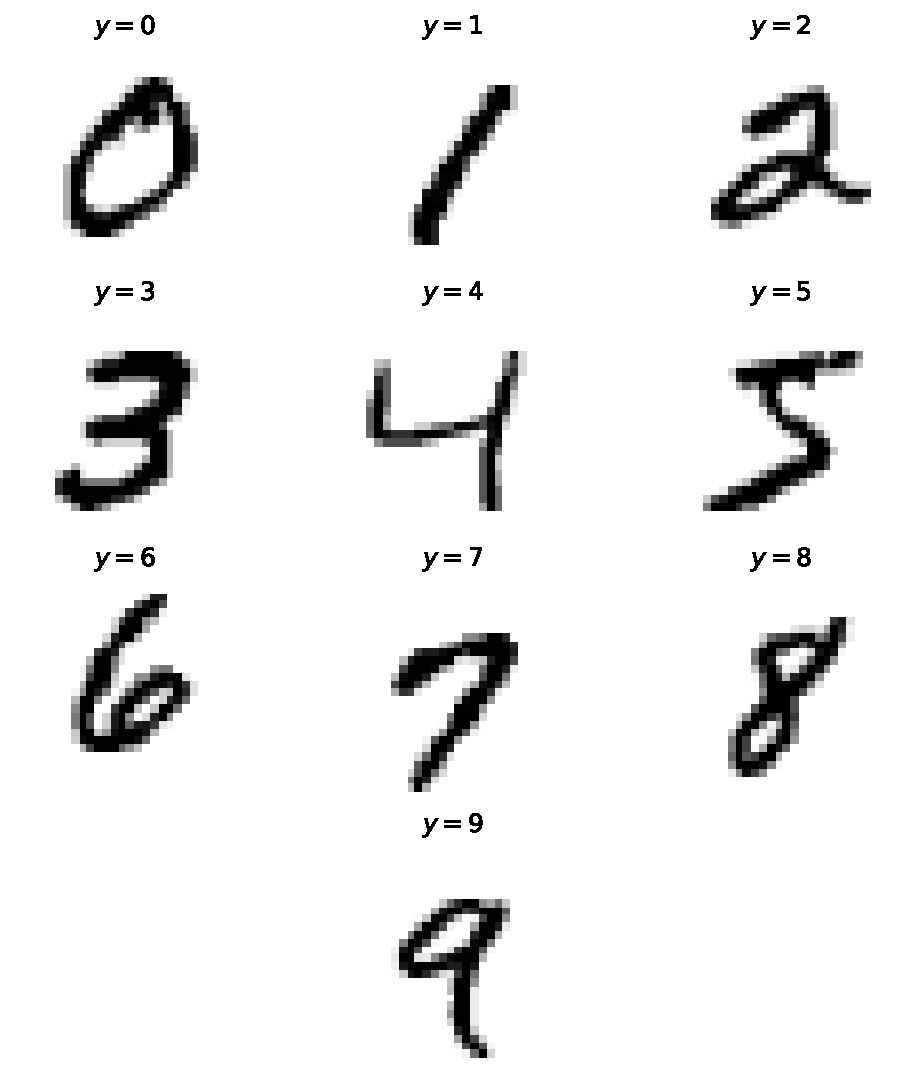
\includegraphics[width=0.5\linewidth]{figs/ex4_2_digits}
		\caption{Samples from the 10 different classes}
		\label{fig:ex4_2_digits}
	\end{figure}
	
	\subsection*{SVC}
	
	The SVC with RBF kernel trained on the whole training set achieved a final accuracy on test set of \SI{97.92}{\percent}.
	
	\subsection*{Neural network classifier}
	
	The neural network architecture is shown in \prettyref{fig:ex4_2_network}, the model summary is shown below.
	
	For the Conv1 layer a kernel size of $4\cross4$, $16$ filters and a stride of $(2,2)$ was used.
	For the Conv2 layer a kernel size of $3\cross3$, $16$ filters and a stride of $(2,2)$ was used.
	For the Conv3 layer a kernel size of $3\cross3$, $32$ filters and a stride of $(1,1)$ was used. 
	
	All layers, except the Output layer use a \texttt{ReLu} activation.
	The dropout layers use a drop rate of $0.5$.
	
	For the Output layer a linear activation was used. The predicted label is then decided by selecting the highest of the $10$ output values. Another approach would be to use a softmax activation on the output. This has the advantage, that the outputs can then be interpreted as probabilities.
	
	Using the same notation is in Problem 4.1 the number of parameters can be computed by accounting for the weights of one kernel $M_\mathrm{h} M_\mathrm{w}$ both for each input and each output channel $M_\mathrm{h} M_\mathrm{w} c_\mathrm{i} c_\mathrm{o}$ and the $c_\mathrm{o}$ bias terms.
	In total 
	\begin{equation}
		M_\mathrm{h} M_\mathrm{w} c_\mathrm{i} c_\mathrm{o} + c_\mathrm{o}.
	\end{equation}
	For example for Conv3 $M_\mathrm{h}=M_\mathrm{w}=3$, $c_\mathrm{i}=16$, $c_\mathrm{o}=32$ adding up to $3\cross3\cross16\cross32+32=4640$ parameters.
	
	For the Dense1 layer it is $512\cross256+512$ due to the $512$ input and $256$ output size.
	
	For padding set to valid the output height is given by
	\begin{equation}
		h_\mathrm{o} = \mathrm{floor}\left( \frac{h_\mathrm{i}-M_\mathrm{h}}{\mathrm{stride}}+1 \right).
	\end{equation}
	The stride is in the denominator as it sets the number of positions the filter is moved each step. The filter height is subtracted from the input height in the numerator because for valid padding no values are added to the input.
	As all my kernels have the same size in both directions and also the stride was set to the same values the width and height are the same at the output of each layer.
	
	\begin{figure}[H]
		\centering
		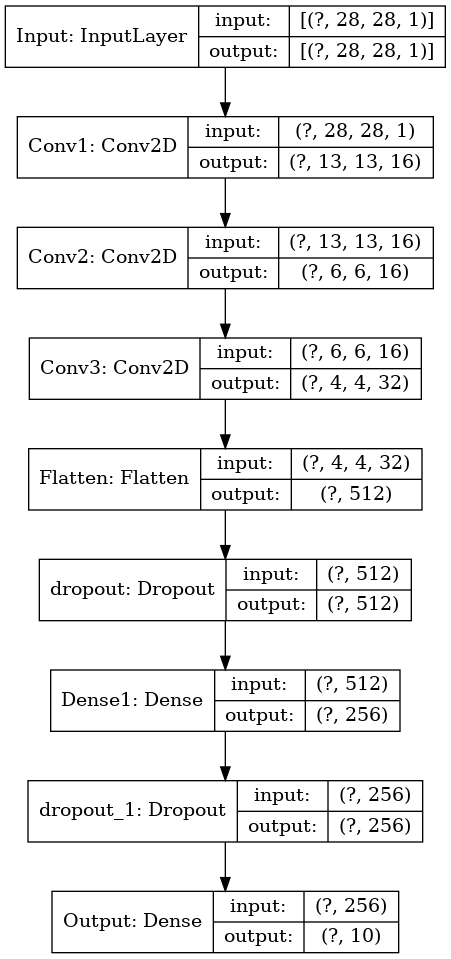
\includegraphics[width=0.3\linewidth]{figs/ex4_2_model.png}
		\caption{Neural network architecture}
		\label{fig:ex4_2_network}
	\end{figure}
	
		\begin{lstlisting}
_________________________________________________________________
Layer (type)                 Output Shape              Param #   
=================================================================
Conv1 (Conv2D)               (None, 13, 13, 16)        272       
_________________________________________________________________
Conv2 (Conv2D)               (None, 6, 6, 16)          2320      
_________________________________________________________________
Conv3 (Conv2D)               (None, 4, 4, 32)          4640      
_________________________________________________________________
Flatten (Flatten)            (None, 512)               0         
_________________________________________________________________
dropout (Dropout)            (None, 512)               0         
_________________________________________________________________
Dense1 (Dense)               (None, 256)               131328    
_________________________________________________________________
dropout_1 (Dropout)          (None, 256)               0         
_________________________________________________________________
Output (Dense)               (None, 10)                2570      
=================================================================
Total params: 141,130
Trainable params: 141,130
Non-trainable params: 0
_________________________________________________________________
	\end{lstlisting}
	
	The batch size was set to $64$, the number of epochs to $20$ and the Adam optimizer has been used. \texttt{CategoricalCrossEntropy} has been used as a loss function. When the final layer is a linear layer the option \texttt{from\_logits} has to be set to true. If a softmax layer were to be used this option has to be set to false. 
	
	The learning curve is shown in \prettyref{fig:ex4_2_learning_curve}. The performance is better on the test set because dropout is not active when evaluating the performance on the test set. The final accuracy on the test set is \SI{99.18}{\percent}.
	
	\begin{figure}[H]
		\centering
		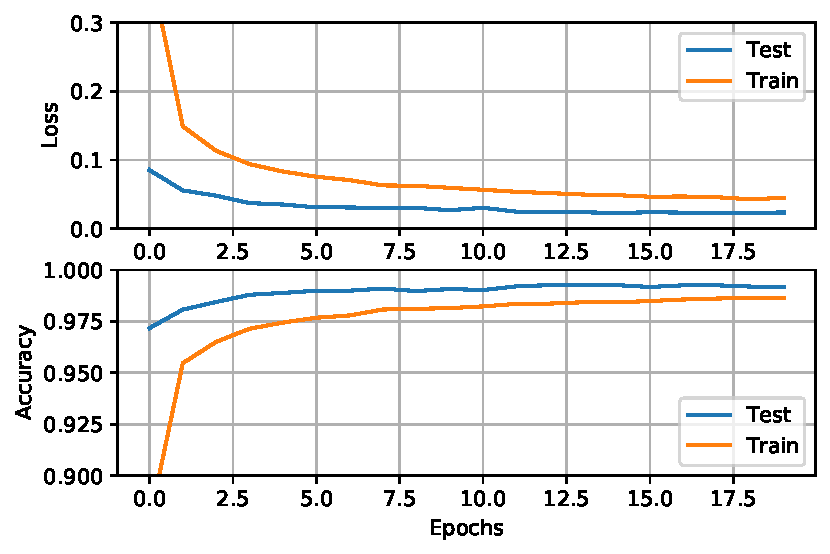
\includegraphics[width=0.75\linewidth]{figs/ex4_2_learning_curve}
		\caption{Learning curves}
		\label{fig:ex4_2_learning_curve}
	\end{figure}
	
	Some samples that have not been classified correctly are shown in \prettyref{fig:ex4_2_incorrect} with the predicted and true labels. The multiclass confusion matrix is shown in \prettyref{tab:ex4_2_confusion}.
	For example $9$ of the samples that are actually $5$ get classified as a $3$, this is the most common error.
	
	Samples with label $5$ are the ones that get misclassified most often with $13$ out of $879$ (\SI{1.48}{\percent}).
	On the samples with label $1$ the highest accuracy is achieved with only $3$ out of $1132$ misclassified (\SI{0.27}{\percent}).
	
	
	\begin{figure}[H]
		\centering
		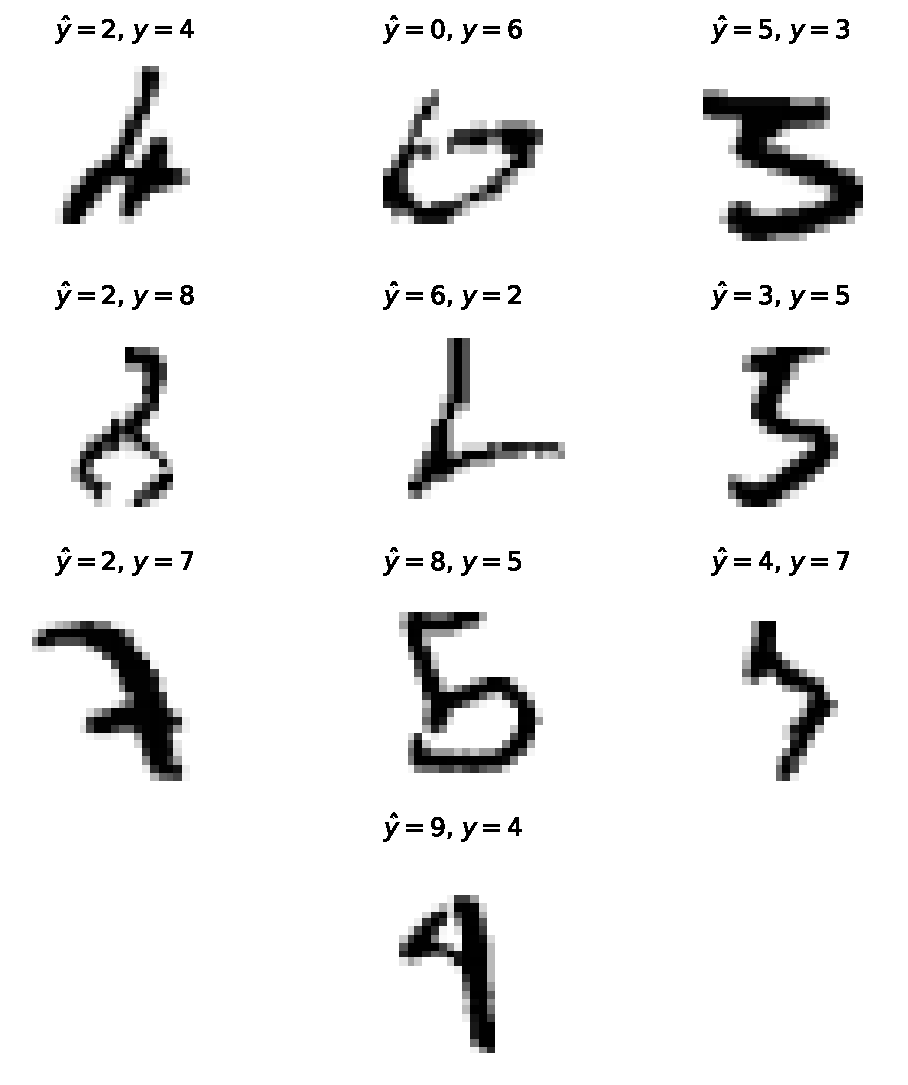
\includegraphics[width=0.5\linewidth]{figs/ex4_2_incorrect}
		\caption{Incorrectly classified samples}
		\label{fig:ex4_2_incorrect}
	\end{figure}
	
	
	
	\begin{table}[H]
		\centering
		\begin{tabular}{|c|c|c|c|c|c|c|c|c|c|c|}
			\hline
			\diagbox{$y$}{$\hat{y}$} & 0   & 1    & 2    & 3    & 4   & 5   & 6   & 7    & 8   & 9   \\ \hline
			0              & 977 & 0    & 1    & 0    & 0   & 0   & 1   & 1    & 0   & 0   \\ \hline
			1              & 0   & 1132 & 1    & 0    & 0   & 0   & 1   & 1    & 0   & 0   \\ \hline
			2              & 0   & 0    & 1027 & 0    & 1   & 0   & 3   & 1    & 0   & 0   \\ \hline
			3              & 0   & 0    & 1    & 1003 & 0   & 3   & 0   & 2    & 1   & 0   \\ \hline
			4              & 0   & 0    & 1    & 0    & 975 & 0   & 2   & 0    & 0   & 4   \\ \hline
			5              & 0   & 0    & 0    & 9    & 0   & 879 & 1   & 1    & 1   & 1   \\ \hline
			6              & 3   & 2    & 0    & 0    & 1   & 1   & 950 & 0    & 1   & 0   \\ \hline
			7              & 0   & 2    & 6    & 0    & 1   & 0   & 0   & 1018 & 0   & 1   \\ \hline
			8              & 3   & 1    & 3    & 1    & 0   & 0   & 0   & 1    & 962 & 3   \\ \hline
			9              & 0   & 2    & 0    & 2    & 5   & 0   & 0   & 5    & 0   & 995 \\ \hline
		\end{tabular}
		\caption{Confusion Matrix}
		\label{tab:ex4_2_confusion}
	\end{table}
	
	An input sample and the $5$ filtered outputs after the first and last convolutional layer are shown in \prettyref{fig:ex4_2_features}. The first layer acts as a feature extractor as can be seen in the plots. For example the middle filter extracts the horizontal line of the input.
	After the third convolutional layer the size is only $4\cross4$ and the original image is not recognizable anymore.
	
	\begin{figure}[H]
		\centering	
		\subfloat[Input]{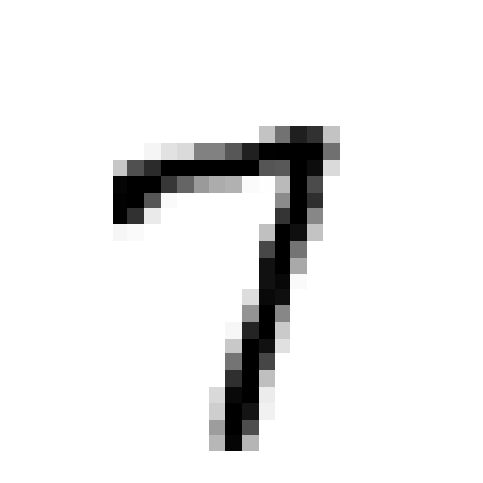
\includegraphics[width = 0.15\linewidth]{figs/ex4_2_inp}}\\
		\subfloat[Output after Conv1 Layer]{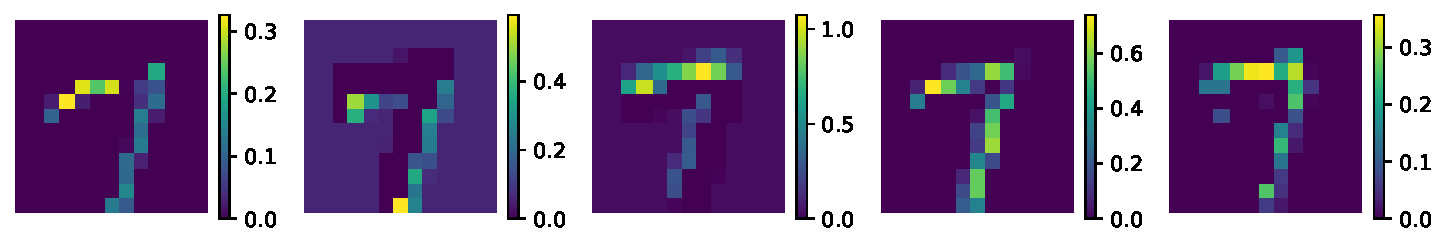
\includegraphics[width=0.75\linewidth]{figs/ex4_2_features1}} \\
		\subfloat[Output after Conv3 Layer]{	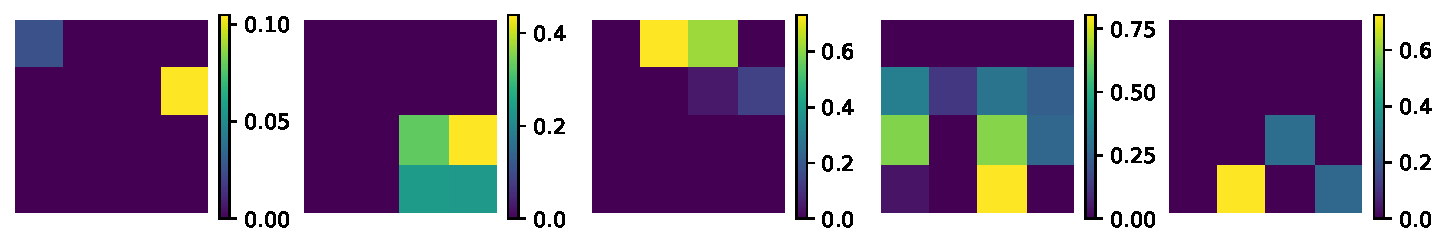
\includegraphics[width=0.75\linewidth]{figs/ex4_2_features2}}
		\caption{Heatmap of the output after the first and last convolutional layer}
		\label{fig:ex4_2_features}
	\end{figure}
	
	\section*{Problem 4.3}
	
	\subsection*{kMeans}
	
	Clustering results for different values of $k$ with the standard kMeans algorithm are shown in \prettyref{fig:ex4_3_clustering}. In \prettyref{fig:ex4_3_different} a different result for $k=4$ is shown, indicating that kMeans does not always converge to the same solution. The clustering result depends on the initial centroids. If the initialization is poor kMeans can get stuck in a local minimum leading to a different result.
	
	
	\begin{figure}[H]
		\centering	
		\subfloat[$k=2$]{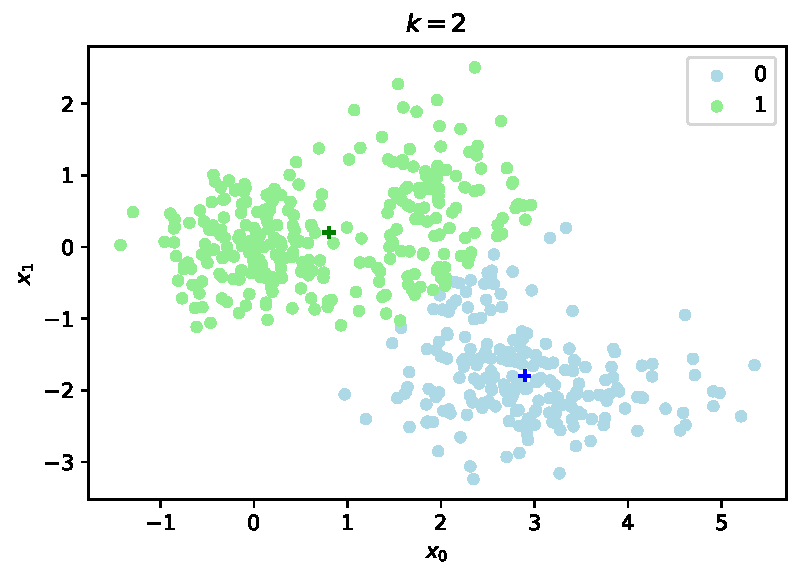
\includegraphics[width=0.33\linewidth]{figs/ex4_3_k2}}
		\subfloat[$k=3$]{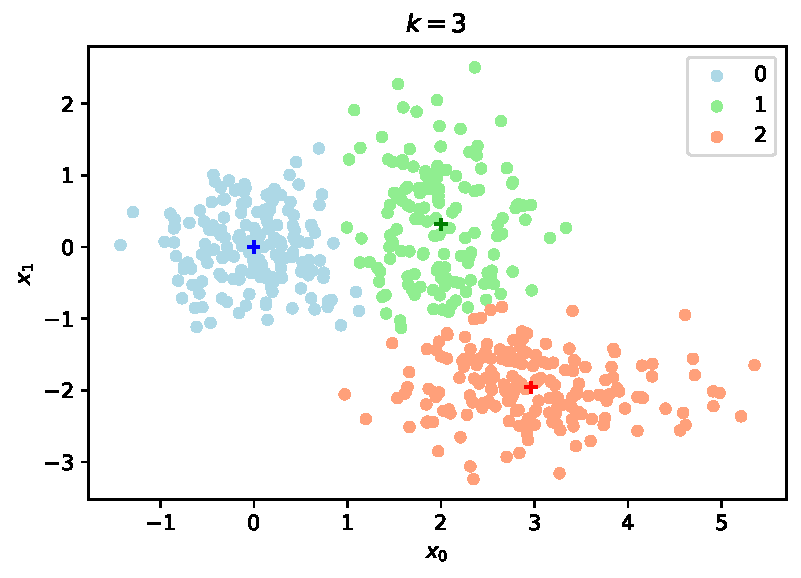
\includegraphics[width=0.33\linewidth]{figs/ex4_3_k3}}
		\subfloat[$k=4$]{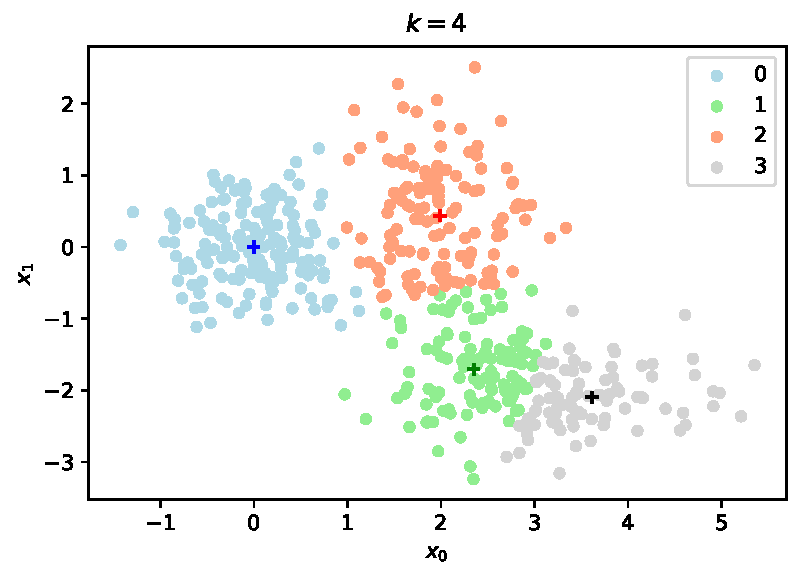
\includegraphics[width=0.33\linewidth]{figs/ex4_3_k4}}
		\caption{Clustering results for different $k$}
		\label{fig:ex4_3_clustering}
	\end{figure}
	
	\begin{figure}[H]
		\centering
		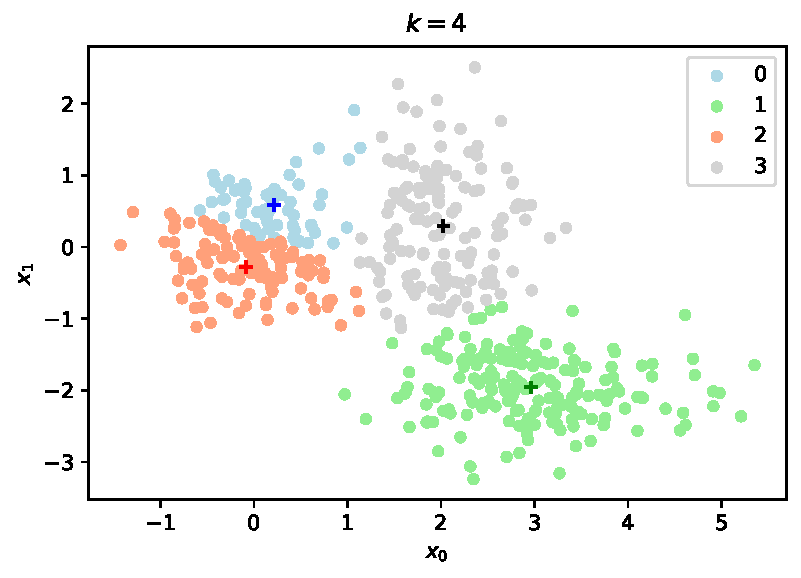
\includegraphics[width=0.33\linewidth]{figs/ex4_3_k4_different}
		\caption{Different clustering results for $k=4$}
		\label{fig:ex4_3_different}
	\end{figure}
	
	Samples from the region $x_0>4$ have been selected to obtain the visualization of the training process in \prettyref{fig:ex4_3_km_iter}. This poor choice of initialization leads to a high number of iterations needed until the algorithm converges. The cluster centroids move little by little during iteration.
	
	\begin{figure}[H]
		\centering
		\foreach \x in {0,1,2,3,4,5,6,7,8,9,10,11,12,13,14,15,16,17}
		{
			\subfloat{\includegraphics[width=0.3\linewidth]{figs/ex4_3_k_iter_\x.pdf}}
		}
		\caption{kMeans Iteration}
		\label{fig:ex4_3_km_iter}
	\end{figure}
	
	
	
	\subsection*{kMeans++}
	
	To overcome the issues of the standard kMeans algorithm the kMeans++ algorithm has been implemented. It uses a different initialization scheme where samples close to an already selected centroid are less likely to be chosen. This should prevent such poor initializations as shown above.
	
	The visualization is shown in \prettyref{fig:ex4_3_kmpp_iter} it can be seen that the initial selection is already a good estimate. It takes just five iterations for the algorithm to converge in this case. 	
	
		\begin{figure}[H]
		\centering
		\foreach \x in {0,1,2,3,4,5}
		{
			\subfloat{\includegraphics[width=0.3\linewidth]{figs/ex4_3_kpp_iter_\x.pdf}}
		}
		\caption{kMeans++ Iteration}
		\label{fig:ex4_3_kmpp_iter}
	\end{figure}
	
	
	\subsection*{MNIST Clustering}
	
	The kMeans++ method has been tested on the MNIST dataset. A histogram of the assigned cluster labels and the true labels is shown in \prettyref{fig:ex4_3_histogram}. The true labels are almost evenly distributed whereas with the clustering e.g. six is assigned less frequent.
	
	\begin{figure}[H]
		\centering
		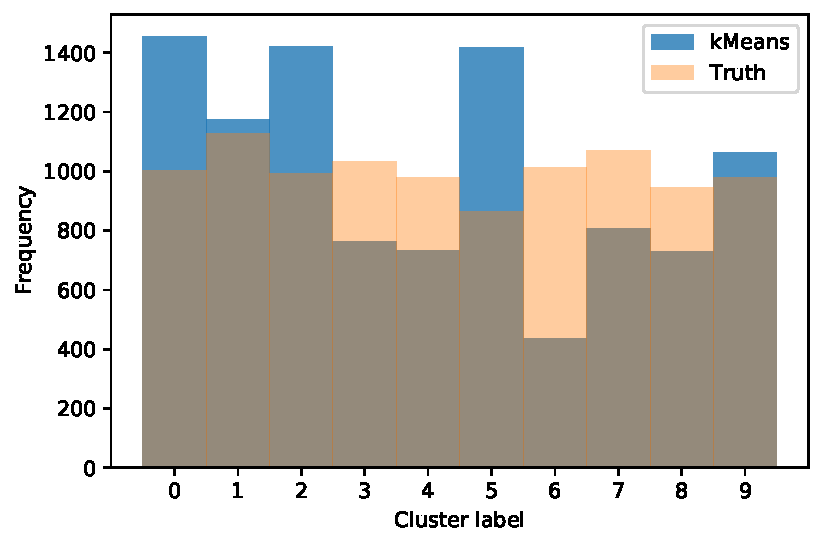
\includegraphics[width=0.5\linewidth]{figs/ex4_3_hist}
		\caption{Histogram of predicted and true cluster labels in the dataset}
		\label{fig:ex4_3_histogram}
	\end{figure}
	
	The $k=10$ centroids are shown in \prettyref{fig:ex4_3_centroids} and the assigned labels $\hat{y}$ on top. The labels have been assigned by finding the most frequent true label in the corresponding cluster. 
	It can be seen that some centroids have the same $\hat{y}$ e.g. $1$ and $6$ meaning that kMeans wasn't able to cluster the samples correctly.
	
	\begin{figure}[H]
		\centering
		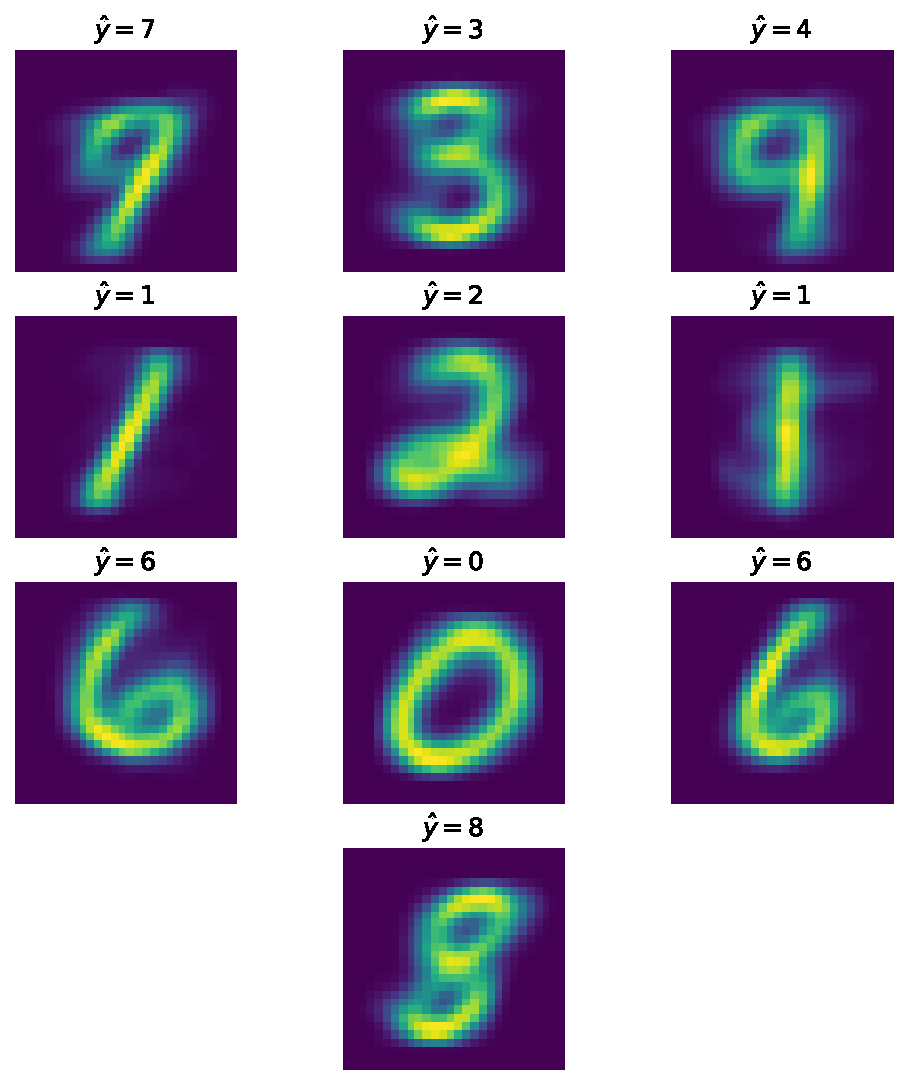
\includegraphics[width=0.5\linewidth]{figs/ex4_3_centroids}
		\caption{Centroids}
		\label{fig:ex4_3_centroids}
	\end{figure}
	

	

\end{document}